\section{Methodology}
\label{sec:method}

In this section, we present a generalized framework for computing the
active subspace. The framework is employed to the H$_2$/O$_2$ reaction kinetics
problem whereby the 
pre-exponent ($A_i$) in the rate law associated with individual reactions provided in
Table~\ref{tab:kinetics} is considered to be uniformly
distributed in the interval, $[0.9A_i^\ast, 1.1A_i^\ast]$; $A_i^\ast$ is the nominal
estimate provided in~\cite{Yetter:1991}.
Specifically, we employed two strategies --
a perturbation-based strategy that involves computation of model
gradients using finite difference in order to construct the matrix $\hat{\mat{C}}$
in~\eqref{eq:chat}, and a regression-based approach 
that involves a linear approximation of
the model output to approximate the gradient. 
The two approaches are based on Algorithms~1.1 and 1.2 in~\cite{Constantine:2015} and
essentially differ in the way the gradient is estimated. They were implemented in an
iterative manner to ensure computational efficiency by avoiding 
unnecessary model evaluations once a converged active subspace
was achieved. 

%\subsection{Gradient-based approach}
%\label{sub:grad}

As discussed earlier, gradient estimation using finite difference in the 
perturbation-based strategy requires additional model evaluations at the
neighboring points in the input domain. 
Hence, for $N$ samples in a $d$-dimensional parameter space, $N(d+1)$
model evaluations are needed. On the other hand, the regression-based
strategy uses the available set of $N$ model evaluations to approximate
the gradient. The computational effort is therefore 
reduced by a factor $(d+1)$ in this case. The specific sequence of steps
for computing the active subspace is discussed as follows.   

We begin by evaluating the gradient of the model output, $\nabla_{\bm{\xi}}f$,
at an initial set of $n_0$ samples denoted by $\bm{\xi}_i$, $i$ = $1,\ldots,n_0$.
Using the gradient
evaluations, the matrix, $\hat{\mat{C}}$ is computed. Eigenvalue decomposition
of $\hat{\mat{C}}$ yields an initial estimate of the dominant eigenspace,
$\hat{\mat{W}}_1$ and the set of corresponding eigenvalues, 
$\hat{\mat{\Lambda}}_1$. Note that $\hat{\mat{W}}_1$ is obtained by
partitioning the eigenspace around $\lambda_j$ such that the ratio of
subsequent eigenvalues,
$\left(\frac{\lambda_j}{\lambda_{j+1}}\right)>\mathcal{O}(10^2)$.
 At each subsequent iteration, model evaluations are
generated at a new set of $n_k$ samples. The new set of gradient evaluations
are augmented with the available set to re-construct $\hat{\mat{C}}$ followed
by its eigenvalue decomposition. The relative change in the norm of the
difference in squared value of individual components of the dominant
eigenvectors between subsequent iterations is evaluated. The process is
terminated and the resulting eigenspace is considered to have converged once
the maximum relative change at iteration $k$, $\delta \hat{\mat{W}}_{1,j}^{(k)}$
($j$ is used as an index for the eigenvectors),
is smaller than a given tolerance, $\tau$.  A regression fit to
$G(\hat{\mat{W}}_1^\top\bm{\xi})$ is used as a surrogate to characterize and
quantify the uncertainty in the model output. Moreover, the components of the
dominant eigenvectors are used to compute the activity scores, $\bm{\nu}_r(f)$,
which provide an insight into the relative importance of the uncertain inputs.
Note that the index, $r$, corresponds to the number of dominant eigenvectors in
$\hat{\mat{W}}_1$. The sequence of steps as discussed are outlined
in Algorithm~\ref{alg:grad}.

%% Grad-based algorithm

\bigskip
\begin{breakablealgorithm}
\renewcommand{\algorithmicrequire}{\textbf{Input:}}
\renewcommand{\algorithmicensure}{\textbf{Output:}}
  \caption{An iterative strategy for discovering the active subspace}
  \begin{algorithmic}[1]
\Require $\theta_l$, $\theta_u$, $\tau$. 
\Ensure $\hat{\mat{\Lambda}}$, $\hat{\mat{W}}$, $\bm{\nu}_r(f)$ %$\eta$. %
    \Procedure{Active Subspace Computation}{}
    \State Set $k$ = 0
	\State Draw $n_k$ random samples, $\{\bm{\xi}_i\}_{i=1}^{n_k}$ 
         according to $\pi_{\bm{\xi}}$. 
    \State Set $N_\text{total}$ = $n_k$ 
	\iffalse \State Project to the physical space:
        $\{\bm{\theta}_k\}_{k=1}^{n_r}=\theta_l+0.5(\theta_u-\theta_l)\{\bm{\xi}_k\}_{k=1}^{n_r}$ \fi
	\State For each $i=1, \ldots, N_\text{total}$, compute $f(\bm{\xi}_i)$ and the gradient $\bm{g}^i = \nabla_{\bm{\xi}}f(\bm{\xi}_i)$
    \iffalse  
	\Statex\hspace{5mm} Using Finite Difference: 
	\Statex\hspace{5mm} i. Assign a small increment, $d\xi$.
	\Statex\hspace{5mm} ii. Augment the set of samples with neighboring points.
	\be \{\bm{\Xi}_k\}_{k=1}^{n_1(N_p+1)}:~\{\bm{\xi}_k\}_{k=1}^{n_1} \cup
        \{\xi_{k,j}+d\xi\}_{j=1}^{N_p} \nonumber
	\ee
	\Statex\hspace{5mm} iii. Project to the physical space:
        $\{\bm{\theta}_k\}_{k=1}^{n_1(N_p+1)}=\theta_l+0.5(\theta_u-\theta_l)\{\bm{\Xi}_k\}_{k=1}^{n_1(N_p+1)}$
	\Statex\hspace{5mm} iv. Using the augmented set, $\{\bm{\theta}_k\}_{k=1}^{n_1(N_p+1)}$
         compute $\bm{g}^i$.
         \fi 
	\State Compute $\hat{\mat{C}}$ and its eigenvalue decomposition 
		$\hat{\mat{C}}$= $\frac{1}{N_\text{total}}\sum\limits_{i=1}^{N_\text{total}}[\bm{g}^i][\bm{g}^i]^\top$ = 
		$\hat{\mat{W}}^{(k)}\hat{\mat{\Lambda}}^{(k)} \hat{\mat{W}}^{(k)\top}$
	%\State Eigenvalue decomposition, $\mat{C}$ = $W^{(0)}\Lambda^{(0)} W^{(0)\top}$%
	\State Partition: $\hat{\mat{\Lambda}}^{(k)}=
        \begin{bmatrix} \hat{\mat{\Lambda}}_1^{(k)} & \\ & \hat{\mat{\Lambda}}_2^{(k)} \end{bmatrix}$, 
        $\hat{\mat{W}}^{(k)}=\begin{bmatrix} \hat{\mat{W}}_1^{(k)} & \hat{\mat{W}}_2^{(k)} \end{bmatrix}$, 
        $\hat{\mat{\Lambda}}_1^{(k)}\in \mathbb{R}^{N_p\times r}$
	\Loop
		\State Set $k$ = $k$ + 1
		\State Draw $n_k =  \lceil\beta n_{k-1}\rceil$  new random samples 
                $\{\bm{\xi}_i\}_{i=1}^{n_k}$  $\beta\in[0,1]$
                
	%	\State Project $\bm{\xi}_k$~$\rightarrow$~$\bm{\theta}_k$.%
		\State Set $N_\text{total}$ = $N_\text{total}$ + $n_k$ 
		\State Compute $\bm{g}^i = \nabla_{\bm{\xi}_i}f(\bm{\xi}_i)$, 
             	$i=n_{k-1}+1, \ldots, n_{k-1}+n_k$.  
		\State Compute $\hat{\mat{C}}$ = 
        	$\frac{1}{N_\text{total}}\sum\limits_{k=1}^{N_\text{total}}[\bm{g}^i][\bm{g}^i]^\top$
		\State Eigenvalue decomposition, $\hat{\mat{C}}$ = $\hat{\mat{W}}^{(k)}\hat{\mat{\Lambda}}^{(k)}
		 \hat{\mat{W}}^{(k)\top}$
		\State Partition the eigenspace of $\hat{\mat{C}}$ as shown in Step 7
		\State Compute $\delta \hat{\mat{W}}_{1,j}^{(k)}$ = 
                       \scalebox{1.25}{$\frac{\|(\hat{\mat{W}}_{1,j}^{k})^2 - 
                       (\hat{\mat{W}}_{1,j}^{k-1})^2\|}{\|(\hat{\mat{W}}_{1,j}^{k-1})^2\|}$}, 
                       $j = 1,\ldots,r$.
		\If {$\max\left(\delta \hat{\mat{W}}_{1,j}^{(k)}\right)<\tau$}
			\State break
		\EndIf
	\EndLoop
	\State Compute $\nu_{i,r}(f) = \sum\limits_{j=1}^{r} \Lambda_j w_{i,j}^2$,
	$i=1,\ldots,N_p$.
	\State Normalize $\nu_{i,r}(f)$ as $\tilde{\nu}_{i,r}(f)$ = \scalebox{1.25}{$\frac{\nu_{i,r}(f)}{\sum_i\nu_{i,r}(f)}$}.
	
    \EndProcedure
  \end{algorithmic}
  \label{alg:grad}
\end{breakablealgorithm}
\bigskip

To assess its feasibility and suitability, we implement
Algorithm~\ref{alg:grad} to compute the active subspace for 
the 19-dimensional H$_2$/O$_2$ reaction kinetics
problem with uncertain $A_i$'s. For the purpose of verification,
$\hat{\mat{C}}$ was initially constructed using a large set of samples
($N$~=~1000) in the input domain. The gradient was estimated using
finite difference, and hence, a total of 20,000 model runs were performed. 
In Figure~\ref{fig:eig_comp}, we illustrate the comparison of
the resulting normalized eigenvalue spectrum ($\lambda_1, \ldots, 
\lambda_{19}$) with the same using a much 
smaller set of samples, $n$~=~$\{20,40,80,120\}$.
%
\begin{figure}[htbp]
 \begin{center}
  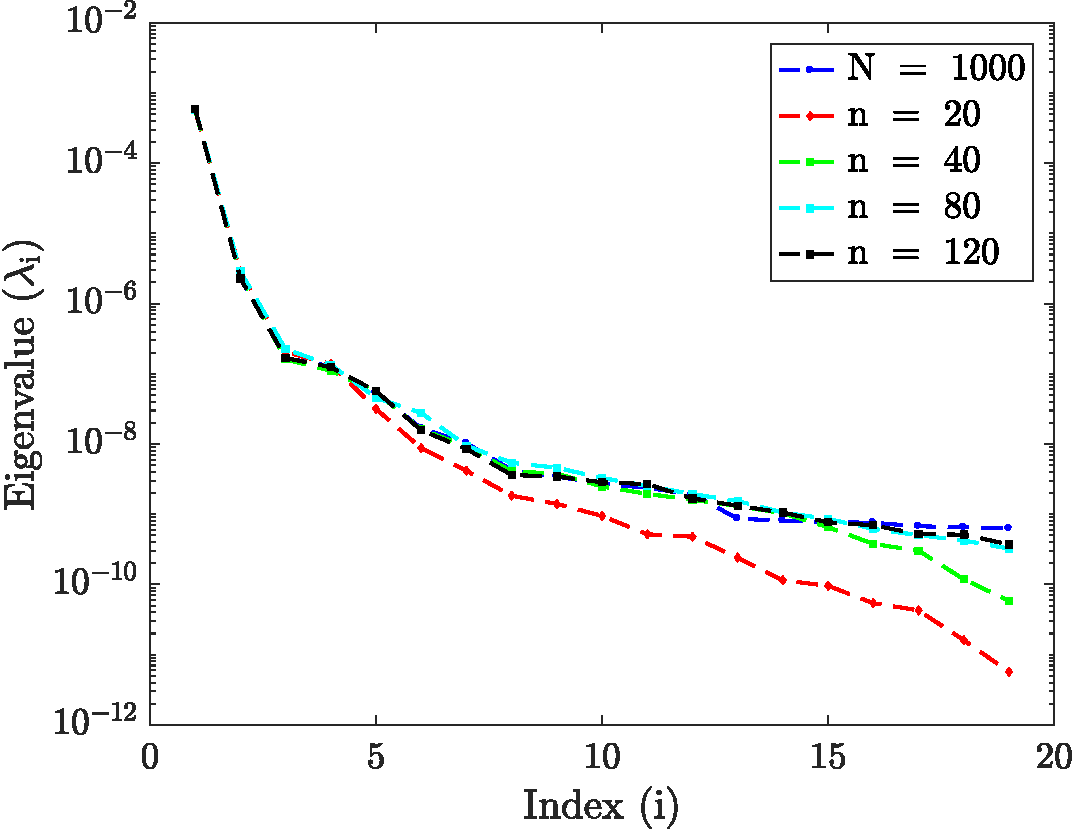
\includegraphics[width=0.45\textwidth]{./Figures/eig_comp}
%   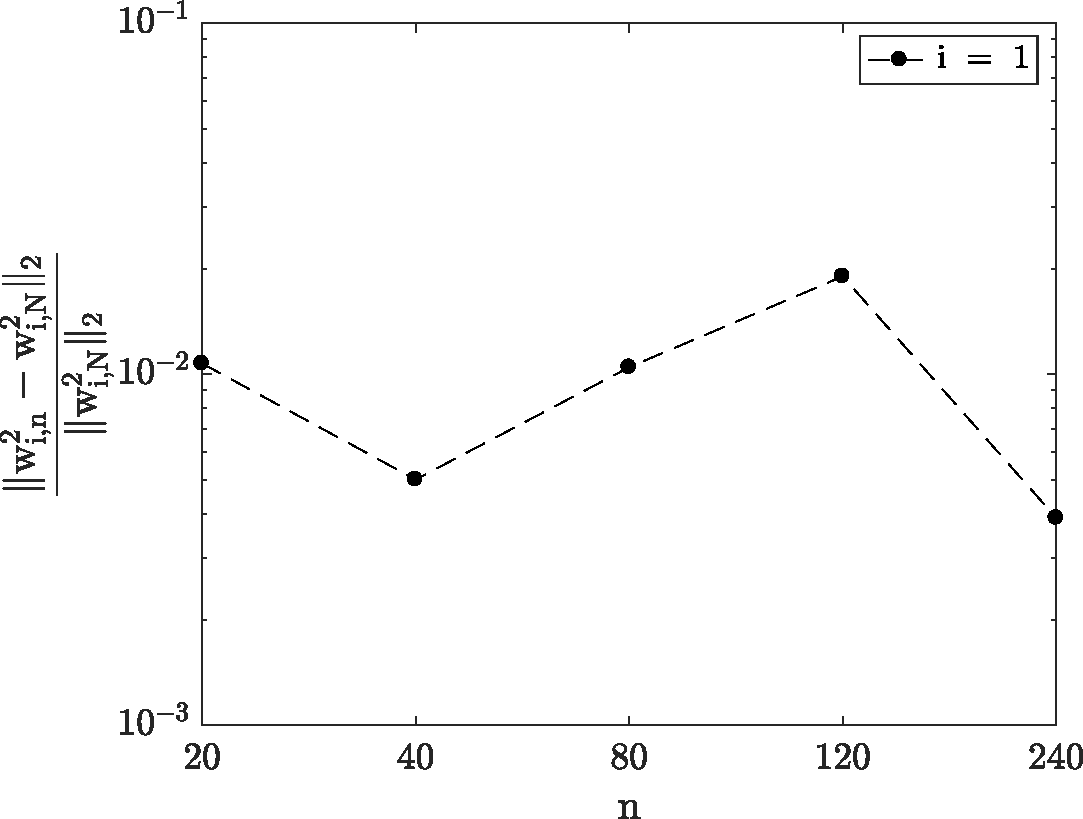
\includegraphics[width=0.48\textwidth]{./Figures/err_eigv_1}
\caption{A comparison of the normalized eigenvalue spectrum using $n$ = $\{20,40,80,120\}$ samples with that
obtained using a much larger sample size, $N$~=~1000. 
%Right: Relative $L_2$ 
%norm of the difference between
%the square of individual components ($w_i$'s) of the dominant eigenvector evaluated using 
$N$=1000 and $n$ = $\{20,40,80,120\}$ samples.
} 
\label{fig:eig_comp}
\end{center}
\end{figure}
%
We observe that the dominant eigenvalues, $\lambda_1, \ldots, \lambda_4$, 
are approximated 
reasonably well with just 20 samples. As expected, the accuracy of higher-order eigenvalues is observed
to improve with the sample size. Since 
$\left(\frac{\lambda_1}{\lambda_2}\right)\gg 1$, we expect 
a 1-dimensional active subspace. Hence, the first eigenvector 
sufficiently captures the uncertainty in
the  model output. To further confirm this, we evaluate a relative L-2 norm of the difference
 ($\varepsilon_\text{L-2}^{N-n}$) between the 
squared value of corresponding components of the dominant eigenvector, computed using $N$~=~1000
and $n$~=~$\{20,40,80,120\}$.  The quantity, $\varepsilon_\text{L-2}^{N-n}$, was found to be 
$\mathcal{O}(10^{-2})$ for $n$ = 20, 40, and 80; and $\mathcal{O}(10^{-3})$ for $n$ = 120.
Thus, even a small sample size, $n$ = 20, seems to approximate the dominant eigenspace with
reasonable accuracy in this case. 
The iterative strategy therefore offers a significant potential for computational advantage. 

%\subsection{Gradient-free approach}
%\label{sub:gradfree}

The active subspace for the 19-dimensional problem was also computed using the regression-based
approach. As discussed earlier, a linear regression fit to the model output was used to
approximate the gradient using the sequence of steps outlined in Algorithm 1.2 
in~\cite{Constantine:2015}. 
%
%The gradient-free approach exploits a regression-based local linear
%approximation to the model output for estimating the gradients, $\bm{g}^i$
%in Algorithm~\ref{alg:grad}. Once again, we use an iterative strategy for
%computing the active subspace for the 19-dimensional 
%H$_2$/O$_2$ reaction kinetics problem considered in~\ref{sub:grad}.
%Moreover, we compare our findings with
%those obtained using the gradient-based approach to assess consistency
%between the two approaches. 
%
%In the gradient-free approach, the model output is first computed at an initial set of $n_0$ samples. 
%An independent set of $M$ samples is also drawn according to the joint probability distribution of the inputs.
%For each sample in $M$, $p$ nearest neighbors in the $n_0$ set are identified. A least-squares fit to model
%evaluations at the $p$ samples is performed. The slope vector ($\bm{b}_i$) of the regression fit is stored
%separately and the process is repeated for each sample in $M$. The symmetric and positive semi-definite matrix,
%$\hat{\mat{C}}$ is constructed using the slope vectors as follows:
%%
%\be
%\hat{\mat{C}} = \frac{1}{M}\sum\limits_{i=1}^{M}\bm{b}_i\bm{b}_i^\top = \hat{\bm{W}}\hat{\bm{\Lambda}}\hat{\bm{W}}^\top
%\ee
%%
%Hence, the gradient-free approach essentially differs in the procedure for constructing the matrix, $\hat{\mat{C}}$.
%Instead of the model evaluations, a linear regression-based approximation is used to estimate the gradient of
%the model output. The suitability of this approach thus depends upon the accuracy of this approximation. 
%The active subspace computation involves the same sequence of steps as outlined previously for the gradient-based 
%approach in Algorithm~\ref{alg:grad}. The procedure for constructing $\hat{\mat{C}}$ using a regression-based
%local linear approximation
%of the model output is provided in Algorithm~\ref{alg:free2}.
%
%\bigskip
%\begin{breakablealgorithm}
%\renewcommand{\algorithmicrequire}{\textbf{Input:}}
%\renewcommand{\algorithmicensure}{\textbf{Output:}}
%  \caption{An iterative gradient-free approach for discovering the active subspace}
%  \begin{algorithmic}[1]
%\Require $\theta_l$, $\theta_u$, $M$, $\tau$. 
%\Ensure $\Lambda$, $W$, $\alpha$ %$\eta$. 
%    \Procedure{Gradient-free}{}
%    \State Set $k$ = 0
%	\State Draw $n_k$ random samples, $\{\bm{\xi}_j\}_{j=1}^{n_k}$
%	\State Set $N_\text{total}$ = $n_k$ 
%	\iffalse \State Project to the physical space:
%        $\{\bm{\theta}_k\}_{i=1}^{n_k}=\theta_l+0.5(\theta_u-\theta_l)\{\bm{\xi}_k\}_{k=1}^{n_r}$
%        \fi
%     \State Draw $M$ random samples, $\{\bm{\nu}_i\}_{i=1}^{M}$ 
%	\State Compute $f(\bm\xi_j)$, $j=1, \ldots, N_\text{total}$.
%	\State Compute the matrix $\mathbb{C}$ and its eigenvalue decomposition using Algorithm 3
%	%\State Eigenvalue decomposition, $\mat{C}$ = $W^{(r)}\Lambda^{(r)} W^{(r)\top}$
%	\State Partition: $\Lambda^{(k)}~=~ 
%        \begin{bmatrix} \Lambda_1^{(k)} & \\ & \Lambda_2^{(k)} \end{bmatrix}$, 
%        $W^{(k)}~=~\begin{bmatrix} W_1^{(k)} & W_2^{(k)} \end{bmatrix}$, 
%        $\Lambda_1^{(k)}\in \mathbb{R}^{d\times\mathcal{S}}$
%	\Loop
%		\State Set $k$ = $k$ + 1
%		\State Draw $n_k =  \beta n_{k-1}$  new random samples 
%		$\{\bm{\xi}_j\}_{j=1}^{n_k}$  $\beta =??$  $j = n_{k-1}+1,\ldots,n_{k-1}+n_k$. 
%        \State $N_\text{total}$ = $N_\text{total}$ + $n_k$    
%	\iffalse	\State Project $\bm{\xi}_k$~$\rightarrow$~$\bm{\theta}_k$. \fi
%		 
%		\State Compute $f(\bm\xi_j)$, $j=n_{k-1}+1, \ldots, n_{k-1}+n_k$.  
%		\State Construct the matrix, $\mat{C}$ and its eigenvalue decomposition
%		\State Compute $\delta W_{1,j}^{(k)}$ = 
%                       \scalebox{1.25}{$\frac{\|(W_{1,j}^{k})^2 - 
%                       (W_{1,j}^{k-1})^2\|}{\|(W_{1,j}^{k-1})^2\|}$}, 
%                       $j = 1,\ldots,\mathcal{S}$.
%		\If {$\max\left(\delta W_{1,j}^{(k)}\right)<\tau$}
%			\State break
%		\EndIf
%	\EndLoop
%	\State Compute $\alpha_i(N_\text{total}) = \sum\limits_{j=1}^{\mathcal{S}} \Lambda_{1_{i,j}}W_{1_{i,j}}^2$,
%	$i=1,\ldots,d$.
%    \EndProcedure
%  \end{algorithmic}
%  \label{alg:free1}
%\end{breakablealgorithm}
%\bigskip
%
%\bigskip
%\begin{breakablealgorithm}
%\renewcommand{\algorithmicrequire}{\textbf{Input:}}
%\renewcommand{\algorithmicensure}{\textbf{Output:}}
%  \caption{Algorithm for constructing the matrix, $\hat{\mat{C}} in~\eqref{eq:chat}$}
%  \begin{algorithmic}[1]
%	\Procedure{Local Linear Approximation}{} 
%	\State Draw $N$ random samples, $\{\bm{\xi}_j\}_{j=1}^{N}$ 
%	according to $\pi_{\bm{\xi}}$.
%	\iffalse \State Project to the physical space:
%	$\{\bm{\theta}_k\}_{k=1}^{N}=\theta_l+0.5(\theta_u-\theta_l)\{\bm{\xi}_k\}_{k=1}^{N}$ \fi
%	\State Compute $f(\bm\xi_j)$, $j=1, \ldots, N$.
%	\State Draw $M$ random samples, $\{\bm{\zeta}_i\}_{i=1}^{M}$
%	according to $\pi_{\bm{\xi}}$.
%	\State Choose an integer $p \leq N$ 
%	\State For each $i=1, \ldots, M$, compute 
%	\[
%	\begin{aligned}
%	\Phi_i &= \{ p \text{ nearest points in } \{\bm{\xi}_j\}_{j=1}^{N} \text{ to } \bm{\zeta}_i\}\\
%	\vspace{-2mm}
%	\Psi_i &= \text{subset of } f(\bm\xi_j) \text{ corresponding to the points in } \Phi_i
%	\end{aligned}
%	\]
%	\State Compute linear least square fits 
%	 $f(\bm\xi_j) \approx c_i + b_i^T\bm{\xi}_j$, \  $\bm{\xi}_j \in \Phi_i, \ f(\bm\xi_j) \in \Psi_i$
%	\State Compute the matrix 
%	\[
%	\hat{\mat{C}} \approx \frac{1}{M} \sum_{i=1}^{M} b_i b_i^T = \hat{\mat{W}}\hat{\mat{\Lambda}}\hat{\mat{W}}^\top
%	\]
%	\EndProcedure
%  \end{algorithmic}
%  \label{alg:free2}
%\end{breakablealgorithm}
%\bigskip
%
In Figure~\ref{fig:comp} (left),
we provide a comparison of the square of individual components of the dominant eigenvector, obtained using the two 
strategies. Additionally, the quantity, $\max(\delta \hat{\mat{W}}_{1,j}^{(r)})$ is also plotted in
Figure~\ref{fig:comp} (right) to illustrate convergence characteristics for the regression-based strategy.
%
\begin{figure}[htbp]
 \begin{center}
  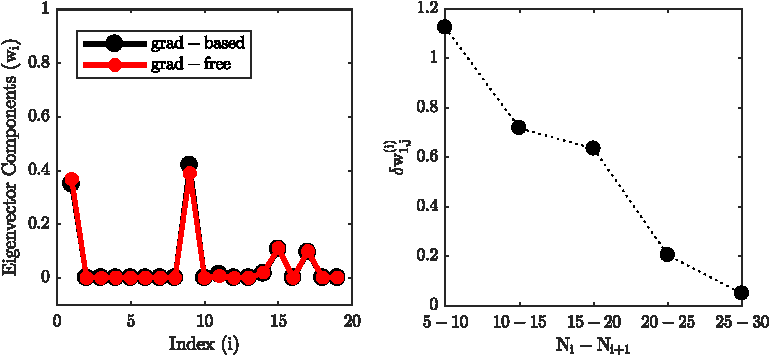
\includegraphics[width=0.8\textwidth]{./Figures/eigv6}
\caption{Left: An illustrative comparison of individual squared components of the converged dominant
eigenvector obtained using the two strategies. Right: The quantity,  $\max(\delta \hat{\mat{W}}_{1,j}^{(r)})$
is plotted for successive iterations to illustrate convergence behavior for the regression-based strategy.}
\label{fig:comp}
\end{center}
\end{figure}
%
Individual components of the dominant eigenvector from the two strategies are observed to be in excellent
agreement with each other. Moreover, as expected,  $\max(\delta \hat{\mat{W}}_{1,j}^{(r)})$ is observed 
to decrease with iterations, and required model evaluations at only 30 samples to converge using $\tau$~=~0.1.

As mentioned earlier, the model output $f(\bm{\xi})$ predominantly varies in the active subspace. Hence, 
$f(\bm{\xi})$ can be approximated as $G(\hat{\mat{W}}_1^\top\bm{\xi})$ in
the subspace. The plot of $G$ versus $\hat{\mat{W}}_1^\top\bm{\xi}$, 
regarded as the \textit{sufficient summary plot} (SSP), obtained using the two strategies is 
compared in Figure~\ref{fig:comp_ssp}.
%
\begin{figure}[htbp]
 \begin{center}
  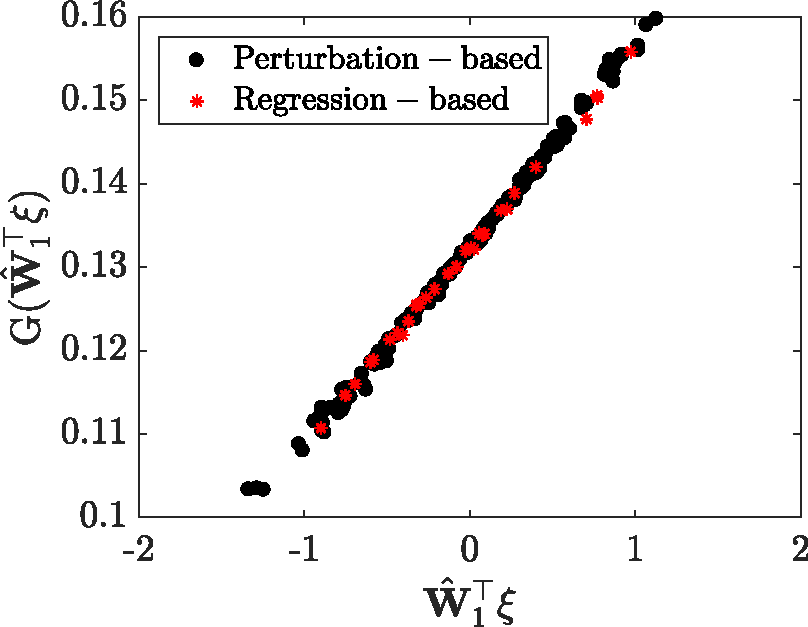
\includegraphics[width=0.45\textwidth]{./Figures/comp_ssp}
\caption{An illustrative comparison of the SSPs generated using the 
perturbation-based and the regression-based strategies for computing the active subspace.}
\label{fig:comp_ssp}
\end{center}
\end{figure}
%
The two SSPs are observed to be in excellent agreement with each other. Moreover, it is interesting to note
that the response in ignition
delay based on the considered prior marginals for $A_i$'s is observed to be approximately linear in the
active subspace. This observation further indicates that the active subspace is 1-dimensional in this case.

We extend the comparative assessment of the two approaches by estimating
the normalized activity scores for individual uncertain inputs ($\tilde{\nu}_{i,r}$; $r$=1 since the
active subspace is 1-dimensional)
using the components of the dominant eigenvector as shown in Algorithm~\ref{alg:grad}.
The activity scores for the 19 uncertain pre-exponents ($A_i$'s), estimated
using the gradient-based and gradient-free approaches are plotted in
Figure~\ref{fig:comp_as} (left).  Additionally, for the purpose of
verification, we compare these estimates with those obtained using the
normalized DGSMs in~\eqref{eq:ndgsm}, as reported in~\cite{Vohra:2018}, in
Figure~\ref{fig:comp_as} (right). 
%
\begin{figure}[htbp]
 \begin{center}
  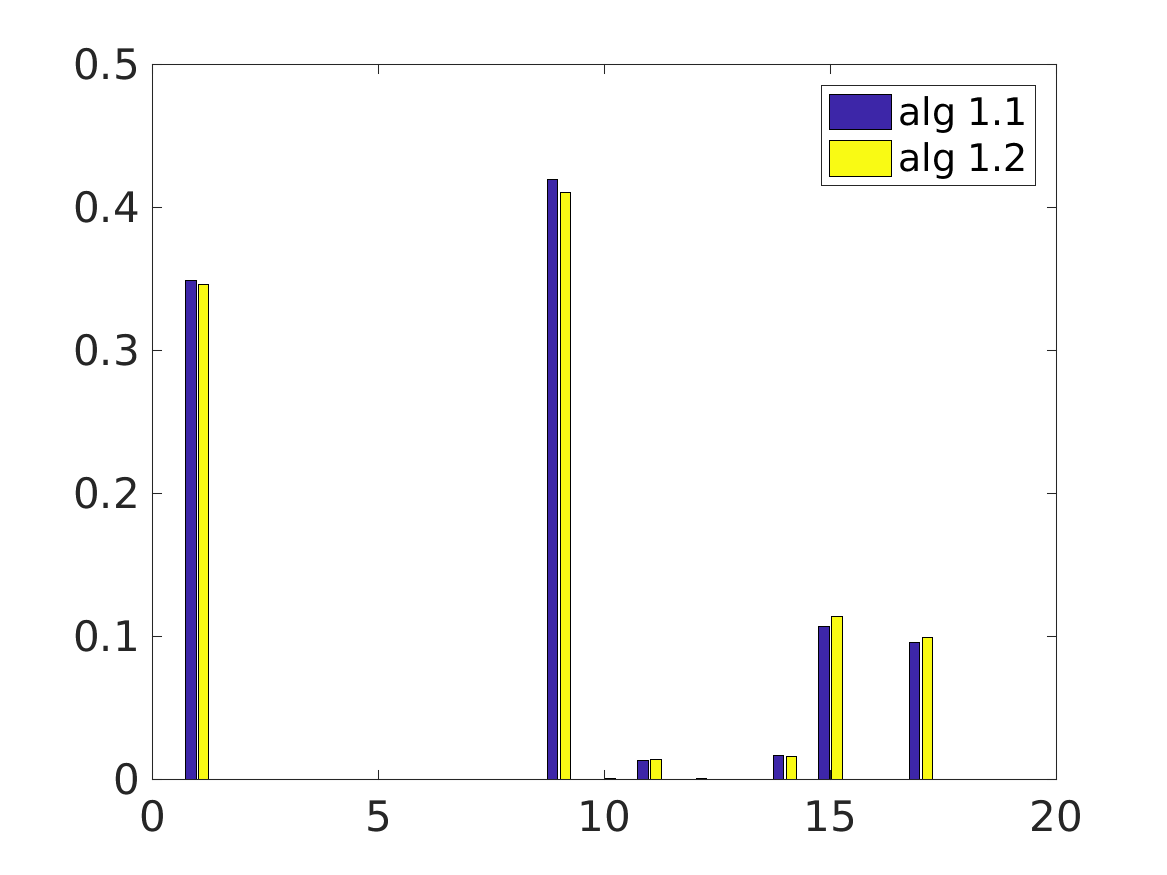
\includegraphics[width=0.45\textwidth]{./Figures/comp_as}
  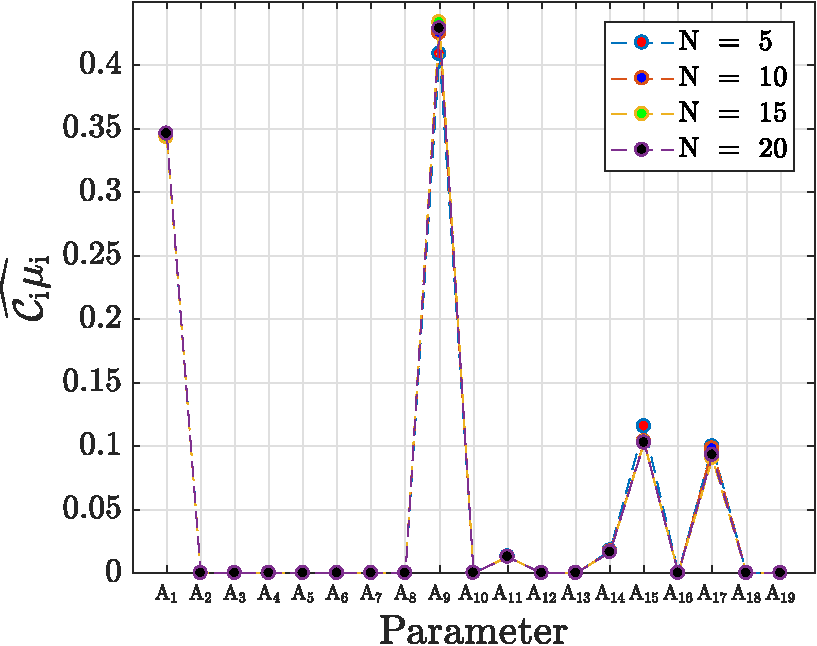
\includegraphics[width=0.45\textwidth]{./Figures/ub_conv_kinetics_rich}
\caption{Left: A bar-graph of normalized activity scores ($\tilde{\nu}_{i,r}$'s) 
for the 19 uncertain pre-exponents ($A_i$'s); $r$
denotes the number of eigenvectors in the active subspace.
Right: A plot of the screening metric ($\tilde{\nu}_i$) for individual $A_i$'s 
(adapted from~\cite{Vohra:2018}).}
\label{fig:comp_as}
\end{center}
\end{figure}
%
The activity scores estimated using the two approaches agree favorably with each other as well as those
based on the screening metric involving the DGSMs from~\cite{Vohra:2018}. It is observed that the uncertainty
associated with the ignition delay is largely due to the uncertainty in $A_9$ and $A_1$. Sensitivity towards
$A_{15}$ and $A_{17}$ is also found to be significant. 

The above comparisons indicate that the two strategies yield consistent results for the 19-dimensional
H$_2$/O$_2$ reaction kinetics problem. In other words, the gradient estimates using pertubation and
regression are reasonably close, and therefore, using the regression-based strategy being computationally
advantageous, would be preferred in this case. In the following section, we shift our focus to 
the higher-dimensional H$_2$/O$_2$ reaction kinetics application involving 33 uncertain inputs. 
